% elementi raccolti dai primi capitoli delle linee guida e dal libro What is the text encoding initiative (Lou Burnard)
% what is the Text Encoding Initiative

\documentclass{beamer}
    
%    \usepackage[english]{babel}
    %\usepackage[latin1]{inputenc}
    %\usepackage[T1]{fontenc}

\mode<presentation>{
  \setbeamertemplate{background canvas}[vertical shading]
  \usetheme{Berkeley}
  \useoutertheme{himinfolines}
}
  
\usepackage{ucs}
\usepackage[utf8]{inputenc}
\usepackage[english,polutonikogreek,italian,UKenglish,british]{babel}
\usepackage{graphicx}
\usepackage{colortbl}
\usepackage{multicol}
\usepackage{ulem}
\usepackage{verbatim}
\usepackage{alltt}
\usepackage{ccicons}
\usepackage{MnSymbol,wasysym}
\usepackage{tikzsymbols}
\usepackage{textcomp}
\usepackage{xmpincl}

\usepackage{parskip}
\setcounter{nframes}{110}
\setcounter{nframe}{1}
\setbeamercovered{dynamic}
\newenvironment{grcenv}{\begin{otherlanguage}{greek}}{\end{otherlanguage}}
\newcommand{\g}[1]{\textgreek{#1}}
\definecolor{darkgreen}{rgb}{0,0.5,0}
\definecolor{darkblue}{rgb}{0,0,0.5}
\definecolor{grey}{rgb}{0.5,0.5,0.5}
\setcounter{tocdepth}{5}

\makeatletter

\makeatother
%\includexmp{LicencesAndLicensing}

%frame00 metadata
    \title{Elementi Codifica TEI}
    \author[A.M. Del Grosso]{Angelo Mario Del Grosso}
    \institute{\texttt{angelo.delgrosso@ilc.cnr.it} \\\bigskip\textit{CNR-ILC-LicoLab} \\\bigskip\url{http://licolab.ilc.cnr.it/}}
    \date{Istituto di Linguistica Computazionale ``A. Zampolli'', \today}
    \AtBeginSection[]{
    \begin{frame}<beamer>
    \addtocounter{nframe}{1}
    \footnotesize
    \frametitle{Progress status}
    \tableofcontents[currentsection,hideothersubsections]
    \end{frame}
    }

\begin{document}

\begin{frame}
	\maketitle
\end{frame}

\begin{frame}
	\frametitle{Sommario della Lezione}
	\tableofcontents
\end{frame}

\section{Introduzione al progetto TEI}

\begin{frame}
	\frametitle{Introduzione}
	\addtocounter{nframe}{1}
    
    %\begin{center}
	%    
\includegraphics[width=.2\textwidth]{../imgs/tei-r.pdf}
	%\end{center}

    \begin{block}{Cos'è la TEI}
        la TEI - \textit{acronimo di Text Encoding Initiative} - rappresenta un punto di riferimento per tutte le iniziative il cui scopo principale è quello di digitalizzare risorse testuali in ambito umanistico per fini di ricerca e di conservazione.
    \end{block}
    
\end{frame}

\begin{frame}
	\frametitle{Introduzione}
	\addtocounter{nframe}{1}
    
    \begin{block}{Qual è l'obiettivo della TEI}
        L'obiettivo della TEI è quello di fornire linee guida per la creazione e la gestione in forma digitale di qualsiasi tipo di dato creato e usato in ambito umanistico.
        \\ E per questo motivo il consorzio investe molte risorse per la accessibilità e la divulgazione della tecnologia che da anni sviluppa.
    \end{block}
    
\end{frame}

\begin{frame}
	\frametitle{Modularità della TEI}
	\addtocounter{nframe}{1}
    
   % \begin{center}
    % 
\includegraphics[width=.2\textwidth]{../imgs/tei-r.pdf}
    % \end{center}

    \begin{itemize}
        
        \item<1-> parleremo del sistema Modulare della TEI
            \begin{itemize}
                \item<1-> Moduli
                \item<1-> Classi
                \item<1-> Macro
                \item<1-> Datatype
            \end{itemize} 
        \item<2-> parleremo degli elementi basilari
            \begin{itemize}
                \item<2-> Intestazione TEI (TEIHeader)
                \item<2-> Elementi e attributi presenti in tutti i documenti TEI
                \item<2-> Esempi di codifica
            \end{itemize} 
    \end{itemize}
    
\end{frame}

\begin{frame}
	\frametitle{I principi fondamentali della TEI}
	\addtocounter{nframe}{1}
    
    \begin{center}
	    
\includegraphics[width=.2\textwidth]{../imgs/tei-r.pdf}
	\end{center}

    \begin{itemize}
        
        \item<1-> Le linee guida della TEI privilegiano il ``significato'' (meaning) del testo piuttosto che l'"aspetto" (layout); privileggia il modello del testo, piuttosto che il formato.
          
        \item<2-> La TEI è stata progettata per essere indipendente dagli strumenti software che la usano per la creazione oppure per l'elaborazione dei documenti elettronici.

        \item<3-> La TEI cresce, matura, si evolve sulla base delle indicazioni e delle ricerche dalla propria comunità di riferimento (community-driven).
           
    \end{itemize}
    
\end{frame}

\section{Infrastruttura TEI}
%% sezione relativa alla infrestruttura TEI

% TEI XML focuses on the meaning of text, rather than its appearance.

% TEI XML can be used for a simple reading-oriented transcription of a primary source, whether that be an authorial manuscript, a printed literary work, an audio broadcast, or a dictionary. It can be used for enriched encodings in which many aspects of such texts are made explicit, so that software of all kinds can operate upon them, from visualisation tools and digital publishing systems to specialised statistical analysis packages. It can be used to provide additional annotations and metadata of all kinds.

% A module is simply a named container for a number of declarations for TEI elements and classes.

% deciding on the proper content for that new element does require some knowledge of the way the TEI system is designed

\begin{frame}
    \frametitle{Infrastruttura TEI}
    \framesubtitle{Tabella Moduli TEI}
    \addtocounter{nframe}{1}
    
    \begin{block}{Formalismi}
	    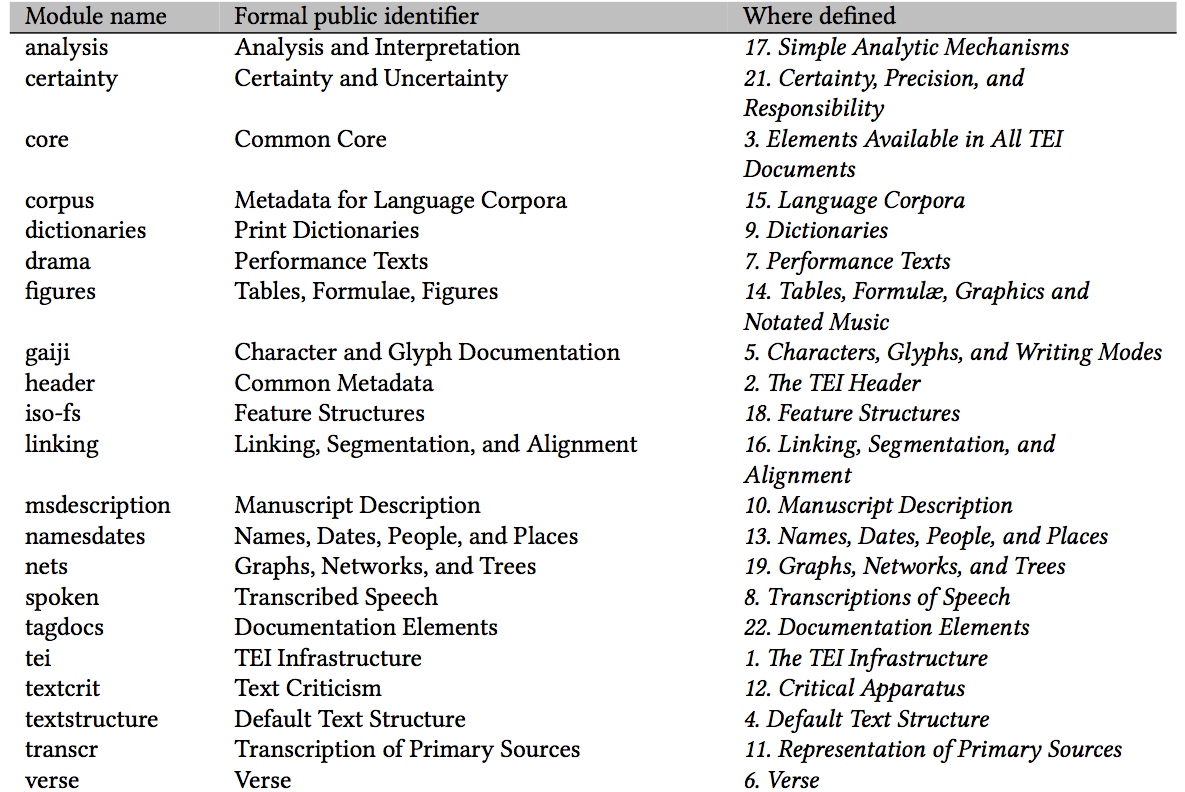
\includegraphics[width=.5\textwidth]{imgs/ModuliTEI.png}
    \end{block}
    

\end{frame}

% xx sezione 1 frame 01
\begin{frame}
    \frametitle{Attributi Globali}
    \framesubtitle{Elenco}
    \addtocounter{nframe}{1}


\textbf{\textrm{att.global} provides attributes common to all elements in the TEI encoding scheme.}

\begin{description}
    \item [@xml:id]     \textbf{identifier} provides a unique identifier for the element bearing the attribute.
    \item [@n]          \textbf{number} gives a number (or other label) for an element, which is not necessarily unique within the document.
    \item [@xml:lang]   \textbf{language} indicates the language of the element content using a ‘tag’ generated according to BCP 47\footnote{see \href{http://google.con}{http://google.com}}.
\end{description}

\end{frame}


% xx sezione 1 frame 02
\begin{frame}
    \frametitle{Attributi Globali}
    \framesubtitle{Elenco cont..}
    \addtocounter{nframe}{1}


\textbf{\textmd{att.global} provides attributes common to all elements in the TEI encoding scheme.}

\begin{description}
    \item rend [att.global.rendition]	(rendition) indicates how the element in question was rendered or presented in the source text.
    \item style [att.global.rendition]	contains an expression in some formal style definition language which defines the rendering or presentation used for this element in the source text
    \item rendition [att.global.rendition]	points to a description of the rendering or presentation used for this element in the source text.
\end{description}

\end{frame}

% xx sezione 1 frame 03
\begin{frame}
    \frametitle{Attributi Globali}
    \framesubtitle{Elenco cont...}
    \addtocounter{nframe}{1}


\textbf{\textmd{att.global} provides attributes common to all elements in the TEI encoding scheme.}

\begin{description}
    \item xml:base	provides a base URI reference with which applications can resolve relative URI references into absolute URI references.
    \item xml:space	signals an intention about how white space should be managed by applications.
    \item source [att.global.source]	specifies the source from which some aspect of this element is drawn.
\end{description}

\end{frame}

% xx sezione 1 frame 04
\begin{frame}
    \frametitle{Attributi Globali}
    \framesubtitle{Elenco cont....}
    \addtocounter{nframe}{1}


\textbf{\textmd{att.global} provides attributes common to all elements in the TEI encoding scheme.}

\begin{description}
    \item  cert [att.global.responsibility]	(certainty) signifies the degree of certainty associated with the intervention or interpretation.
    \item resp [att.global.responsibility]	(responsible party) indicates the agency responsible for the intervention or interpretation, for example an editor or transcriber.
\end{description}

\end{frame}


% xx sezione 1 frame 05

\begin{frame} [fragile]
    \frametitle{Attributi Globali}
    \framesubtitle{Esempio \textrm{@xml:lang}}
    \addtocounter{nframe}{1}

    \textbf{\textrm{xml:lang} indica la lingua e il sistema di scrittura usato}
    \defverbatim{\langatt}{%
        \begin{tiny}
        \begin{verbatim}
            <TEI xmlns="http://www.tei-c.org/ns/1.0">
                <teiHeader xml:lang="en">
                    <!-- ... -->
                </teiHeader>
                <text xml:lang="fr">
                    <body>
                        <div>
                            <!-- chapter one is in French -->
                        </div>
                        <div xml:lang="de">
                            <!-- chapter two is in German -->
                        </div>
                        <div>
                            <!-- chapter three is French -->
                        </div>
                        <!-- ... -->
                    </body>
                </text>
            </TEI>
        \end{verbatim}
        \end{tiny}
        }
        \begin{block}{XML TEI con esempio di uso \textrm{xml:lang} attribute}
            {\langatt}
        \end{block}
\end{frame}


% xx sezione 1 frame 06
\begin{frame}
    \frametitle{Attributi Globali}
    \framesubtitle{Stile e Aspetto}
    \addtocounter{nframe}{1}

    
    \textbf{In the TEI scheme, it is possible to supply information about the appearance of elements within a source document in the following distinct ways:}

    \begin{itemize}
        \item One or more properties may be specified as the default for a set of elements (based on an external scheme, by default CSS), using rendition elements and their selector attributes;
        \item One or more properties may be specified for individual element occurrences, using the rend attribute with any convenient set of one or more sequence-indeterminate tokens;
    \end{itemize}
\end{frame}

% xx sezione 1 frame 07
\begin{frame}
    \frametitle{Attributi Globali}
    \framesubtitle{Stile e Aspetto cont..}
    \addtocounter{nframe}{1}
    
    \textbf{Note that these TEI attributes always describe the rendition or appearance of the source document, not intended output renditions, although often the two may be closely related.}

    \begin{itemize}
        \item One or more properties may be specified for individual element occurrences, using the rendition attribute to point to rendition elements;
        \item One or more properties may be supplied explicitly for individual element occurrences, using the style attribute.
    \end{itemize}

\end{frame}


% xx sezione 1 frame 08

\begin{frame}
    \frametitle{Attributi Globali}
    \framesubtitle{da vari altri Moduli Tabella}
    \addtocounter{nframe}{1}
    %fare una tabella 
class name	module name	see further
att.global.linking	linking	16 Linking, Segmentation, and Alignment
att.global.analytic	analysis	17 Simple Analytic Mechanisms
att.global.facs	transcr	11.1 Digital Facsimiles
att.global.change	transcr	11.7 Identifying Changes and Revisions

\end{frame}

%%%%%%%%%%
% attributi globali: source, cert, resp, xml:base, xml:space
% Altri attributi Globali divisi per classe e per moduli.
% Appendice A per lista alfabetica delle Classi di Modello.

%% Macro e DataType
% Tabella Macro
% 


\section{Intestazione TEI}
%% frame 01
% Every TEI document must have a TEI Header, represented by a <teiHeader> element.
% The TEI header has four main components,
% file description, encoding description, profile description, revision description

% esempio TEI header Minimale
% <teiHeader>
%    <fileDesc>
%        <titleStmt>
%            <title>Title of the work</title>
%        </titleStmt>
%        <publicationStmt>
%            <p>Information about the publication of the work</p>
%        </publicationStmt>
%        <sourceDesc>
%            <p>Information about the source from which the work was derived</p>
%        </sourceDesc>
%    </fileDesc>
% </teiHeader>

% Rifarsi al capitolo due delle linee guida per una descrizione esaustiva e sistematica

\begin{frame}
	\frametitle{Intro Text Encoding Initiative}
	\framesubtitle{Schemi di codifica TEI – Intestazione}
	\addtocounter{nframe}{1}

    \begin{block}{Contenuto del TEI header}
        \textbf{Qualsiasi documento TEI deve includere una intestazione (TEIHeader)}.
    \end{block}

    \begin{block}{TEI header: componenti}
        file description, encoding description, profile description, revision description, no TEI metadata
    \end{block}

\end{frame}

\begin{frame}
	\frametitle{Intro Text Encoding Initiative}
	\framesubtitle{Schemi di codifica TEI – Intestazione}
	\addtocounter{nframe}{1}

    \begin{block}{Contenuto del TEI header}
        \begin{itemize}
            \item metadati relativi al documento (utili per collezioni di testi
            codificati)
            \item descrizione del file usando \texttt{<fileDesc>} (obbligatoria)
            \item descrizioni relative al tipo di codifica, al contenuto del
            documento, alle sue revisioni (facoltative)
        \end{itemize}
    \end{block}
\textit{E' possibile includere testi introduttivi e spiegazioni relative alla
codifica effettuata (preziosi per l’interscambio!)}

\end{frame}



\begin{frame}
	\frametitle{Intro Text Encoding Initiative}
	\framesubtitle{Schemi di codifica TEI – Intestazione}
	\addtocounter{nframe}{1}

    \begin{block}{Testo in prosa}
        Molti elementi dell'intestazione contengono semplicemente del testo in prosa (giunti a qualche livello dell'albero del documento).
    \end{block}

    \begin{block}{Testo in prosa}
       Alcuni elementi possono contenere testo in prosa suddivisa da \textbf{elementi di paragrafo} (\textit{p}), oppure elementi più specifici strutturati, che a loro volta contengono testo in prosa.
    \end{block}
\textit{}

\end{frame}


\begin{frame}
	\frametitle{Intro Text Encoding Initiative}
	\framesubtitle{Schemi di codifica TEI – Intestazione}
	\addtocounter{nframe}{1}

    \begin{block}{Grouping elements}
 
        Gli elementi che terminano con suffisso \textbf{Stmt} (esempio \textit{titleStmt}), racchiudono un gruppo di elementi specifici e specializzati per la codifica di informazioni strutturate.
    \end{block}

    \begin{block}{Grouping elements}
        In molti casi questi elementi possono contenere anche descrizioni con testo in prosa. Ciò permette al curatore della codifica di decidere se utilizzare una strategia strutturata, semi-strutturata o completamente destrutturara.
    \end{block}
\textit{}

\end{frame}


\begin{frame}
	\frametitle{Intro Text Encoding Initiative}
	\framesubtitle{Schemi di codifica TEI – Intestazione}
	\addtocounter{nframe}{1}

    \begin{block}{Dichiarazioni}
        
        Gli elementi che terminano con il suffisso \textbf{Decl} (per esempio \textit{refsDecl}) racchiudono informazioni inerenti specifiche prassi di codifica che sono state usate all'interno del testo digitale.
    \end{block}

    \begin{block}{Dichiarazioni}
        Spesso queste prassi sono descritte in un linguaggio formale, attraverso una serie di dichiarazioni che identificano strutture complesse e descrizioni dettagliate.
    \end{block}

    \textit{Le dichiarazioni possono essere riferite con l'attributo \textbf{decls} per ciascuna parte di testo a cui si applica.}
\textit{}

\end{frame}


\begin{frame}
	\frametitle{Intro Text Encoding Initiative}
	\framesubtitle{Schemi di codifica TEI – Intestazione}
	\addtocounter{nframe}{1}

    \begin{block}{Descrizioni}

        Gli elementi che terminano con il suffisso \textbf{Desc} (esempio \textit{projectDesc}) contengono testo in prosa, che può essere anche strutturata usando specifici elementi.

    \end{block}
\textit{}

\end{frame}


\begin{frame}
	\frametitle{Intro Text Encoding Initiative}
	\framesubtitle{Schemi di codifica TEI – Moduli base}
	\addtocounter{nframe}{1}

	\begin{block}{documento TEI - schema di intestazione TEI minima}
        \texttt{<teiHeader>}
        \\\texttt{ <fileDesc>}
        \\\texttt{  <titleStmt>...</titleStmt>}
        \\\texttt{  <publicationStmt>...</publicationStmt>}
        \\\texttt{  <sourceDesc>...</sourceDesc>}
        \\\texttt{ </fileDesc>}
        \\\texttt{</teiHeader>}
    \end{block}
    

\end{frame}


\begin{frame}
	\frametitle{Intro Text Encoding Initiative}
	\framesubtitle{Schemi di codifica TEI – Intestazione}
	\addtocounter{nframe}{1}

	\begin{block}{documento TEI - schema di intestazione TEI minima}
        Metadati essenziali riguardo il titolo, la modalità di diffusione e
        la fonte originaria di un testo codificato.
        \\Permettono classificazione, archiviazione ed elaborazione
        bibliografica
    \end{block}
    
\end{frame}



\begin{frame}
	\frametitle{Intro Text Encoding Initiative}
	\framesubtitle{Schemi di codifica TEI – Intestazione}
	\addtocounter{nframe}{1}

        \texttt{<teiHeader>
        <fileDesc>
        <titleStmt>
        <title>La Divina Commedia: versione elettronica</title>
        <respStmt>
        <resp>Conversione TEI P5 a cura di</resp><name>M. Rossi</name>
        </respStmt>
        </titleStmt>
        <publicationStmt>
        <publisher>Università di Pisa</publisher>
        <date>2002-11-07</date>
        <availability status=``restricted''><p></p></availability>
        </publicationStmt>
        <sourceDesc>
        <bibl><title>La Divina Commedia</title><author>Dante Alighieri
        </author><publisher>Mondadori</publisher>
        <date>1988</date></bibl>
        </sourceDesc>
        </fileDesc>
        </teiHeader>}

\end{frame}



\begin{frame}
	\frametitle{Intro Text Encoding Initiative}
	\framesubtitle{Schemi di codifica TEI – Intestazione}
	\addtocounter{nframe}{1}

    \begin{block}{Le altre componenti dell’intestazione TEI}
        \begin{itemize}
            \item \texttt{<encodingDesc>} informazioni riguardo lo schema (e il
            modello di codifica) utilizzato
            \item  \texttt{<profileDesc>} descrizione del testo: quando è stato
            creato, da chi, usando quali lingue etc.
            \item \texttt{<revisionDesc>} informazioni sulle versioni del file
        \end{itemize}
    \end{block}
    \textit{I metadati sono una componente essenziale di qualsiasi
        progetto di digitalizzazione}
\end{frame}
\begin{frame}
	\frametitle{Intro Text Encoding Initiative}
	\framesubtitle{Schemi di codifica TEI – Intestazione}
	\addtocounter{nframe}{1}

    \begin{block}{Le altre componenti dell’intestazione TEI}
        \begin{itemize}
            \item elemento \textbf{xenoData}
            \item[] Gli elementi di struttura specifici e specializzati che occorrono all'interno di questo elemento non sono parte del vocabolario TEI. Provengono da altri schemi di metadati come ad esempio il \textit{Dublin Core}.
        \end{itemize}
    \end{block}
    \textit{I metadati sono una componente essenziale di qualsiasi
        progetto di digitalizzazione}
\end{frame}




\begin{frame}
	\frametitle{Intro Text Encoding Initiative}
	\framesubtitle{Schemi di codifica TEI – Moduli base}
	\addtocounter{nframe}{1}

	\begin{block}{Errori frequenti}
        \textit{Si fraintende il significato dell’elemento \texttt{<fileDesc>}}
        \begin{itemize}
            \item serve in primo luogo a dare informazioni sul file stesso, non sul testo originale
            \item il riferimento alla fonte dalla quale è tratto il testo codificato
            deve essere inserito nel \texttt{<sourceDesc>}
        \end{itemize}
    \end{block}

\end{frame}

\begin{frame}
	\frametitle{Intro Text Encoding Initiative}
	\framesubtitle{Schemi di codifica TEI – Intestazione}
	\addtocounter{nframe}{1}

        \textbf{Esempio Intestazione TEI raccomandata}
        \textit{Tratto dalle linee Guida della TEI. Capitolo 2 paragrafo 2.7}
        \\\url{}

\end{frame}

% file description 
%\subsection{File Description}
%
 esempio TEI descrizione file
% tre componenti obbligatorie: title statement, publication statement, descrizione della fonte.

% <titleStmt>
%    <title xml:lang="sk">Yogadarśanam (arthāt yogasūtrapūphah).</title>
%    <title>The Yoga sūtras of Patañjali: a digital edition.</title>
%    <author>Patañjali</author>
%    <funder>Wellcome Institute for the History of Medicine</funder>
%    <principal>Dominik Wujastyk</principal>
%    <respStmt>
%        <name>Wieslaw Mical</name>
%        <resp>data entry and proof</resp>
%    </respStmt>
%    <respStmt> 
%        <name>Jan Hajic</name> 
%        <resp>conversion to TEI-conformant markup</resp> 
%    </respStmt>
% </titleStmt>

% esempio publication statement

%% Descrizione della fonte
% document formally the object or objects from which the TEI document has been derived, using traditional bibliographic
% Born Digital
% Printed Source
% sbobbinatura
% manoscritto (msDesc)

%% Esempio di sourceDesc
% <sourceDesc>
%    <bibl xml:id="Sue1846">
%        <author>
%            <surname>Sue</surname>,
%            <forename>Eugène</forename>
%        </author>
%        <title level="m">Martin, l’enfant trouvé : Mémoires d’un valet de chambre</title>
%        <imprint>
%            <publisher>C. Muquardt</publisher>
%            <pubPlace>Bruxelles</pubPlace>
%            <pubPlace>Leipzig</pubPlace>
%            <date when="1846">MDCCCXLVI</date>
%        </imprint>
%    </bibl>
% </sourceDesc>

% encoding description
%\subsection{Encoding Description}
%% Encoding descsription (<encodingDesc />) is used to supply information about almost any aspect of the encoding process itself

%% esempio descrizione della codifica
% <encodingDesc>
%    <projectDesc>
%        <p>Texts collected for use in the Claremont Shakespeare Clinic, June 1990.</p>
%    </projectDesc>
%    <samplingDecl>
%        <p>Each text contains a sample of up to 2000 words, running from the start of the document to the end of the sentence
%            after the 2000 word mark. For the purposes of word counting, hyphens and apostrophes were treated as spaces.
%            </p>
%    </samplingDecl>
%    <editorialDecl>
%        <normalization>
%            <p>Word forms broken by end of line hyphenation have been reconstructed without comment. The hyphen has been removed
%                except for hyphenated forms attested elsewhere in the text. </p>
%        </normalization>
%        <quotation marks="all" form="std">
%            <p>All quotation marks have been removed. Direct speech is represented by the use of the
%                <gi>said</gi> tag; other quoted material is represented by means of the
%                <gi>q</gi> tag. </p>
%        </quotation>
%    </editorialDecl>
% </encodingDesc>

%% for human reader and for automated process

% esempio charDecl
% <charDecl>
%    <glyph xml:id="z103">
%        <glyphName>LATIN LETTER Z WITH TWO STROKES</glyphName>
%        <mapping type="standardized">z</mapping>
%        <mapping type="PUA">U+E304</mapping>
%    </glyph>
% </charDecl>

% segue nel testo 
% <p> ... mulct<g ref="#z103"/> ... </p>

% tassonomia

% <classDecl>
%    <taxonomy xml:id="size">
%        <category xml:id="large">
%            <catDesc>story occupies more than half a page</catDesc>
%        </category>
%        <category xml:id="medium">
%            <catDesc>story occupies between quarter and a half page</catDesc>
%        </category>
%        <category xml:id="small">
%            <catDesc>story occupies less than a quarter page</catDesc>
%        </category>
%        <!-- etc -->
%    </taxonomy>
%    <taxonomy xml:id="topic">
%        <category xml:id="politics-domestic">
%            <catDesc>Refers to domestic political events</catDesc>
%        </category>
%        <category xml:id="politics-foreign">
%            <catDesc>Refers to foreign political events</catDesc>
%        </category>
%        <category xml:id="social-women">
%            <catDesc>refers to role of women in society</catDesc>
%        </category>
%        <category xml:id="social-servants">
%            <catDesc>refers to role of servants in society</catDesc>
%        </category>
%        <!-- etc -->
%    </taxonomy>
% </classDecl>

% uso nel testo 
% <catRef target="#small #social-women"/>

%% esempio dichiarazione dei tag
% <tagsDecl>
%    <rendition xml:id="IT" scheme="css">font-style:italic</rendition>
%    <rendition xml:id="FontRoman" scheme="css">font-family: serif</rendition>
%    <namespace name="http://www.tei-c.org/ns/1.0">
%        <tagUsage gi="emph" render="#IT" />
%        <tagUsage gi="hi" render="#IT" />
%        <tagUsage gi="text" render="#FontRoman" />
%    </namespace>
% </tagsDecl>

% uso nel testo
% @rendition attribute

% profile description
%\subsection{Profile Description}
%% elemento che descrive il profilo del documento TEI
% elementi di metadatazione non bibliografici
% elementi per edentificare i vari passaggi genetici elemento <listChange />
 %% esempio proust di Pierazzo
 %% esempio carteggio

 %% esempio profile
% <profileDesc>
%    <creation>
%        <date when="1962" /> </creation>
%    <textClass>
%        <catRef target="#WRI #ALLTIM1 #ALLAVA2 #ALLTYP3 #WRIDOM5 #WRILEV2 #WRIMED1 #WRIPP5 #WRISAM3 #WRISTA2 #WRITAS0" />
%        <classCode scheme="DLEE">W nonAc: humanities arts</classCode>
%        <keywords scheme="COPAC">
%            <term>History, Modern - 19th century</term>
%            <term>Capitalism - History - 19th century</term>
%            <term>World, 1848-1875</term>
%        </keywords>
%    </textClass>
% </profileDesc>

% revision description
%\subsection{Revision Description}
%% represented by a <revisionDesc> element which contains a list of <change>
% given first. The <listChange> element mentioned above may also be used here to refer to identified stages in the evolution of the electronic file

% esempio
% <revisionDesc>
%    <listChange>
%        <change when="2013-05-11">First complete draft</change>
%        <change when="2013-04-07">Created header and document structure</change>
%    </listChange>
% </revisionDesc>

% no tei metadata
%\subsection{No TEI Metadata}
%\input{includes/subinclude/noTEIData.tex}


\section{Elementi di base TEI}
% capitoli 3 e 4 delle linee guida e estratti dal libro what is TEI (The structural organization, Varieties of textual structure, parte della TEI cornucopia part 1)
% fare esempio facsimile e codifica dei fenomeni (vedere anche slide del turco e fiormonte-ciotti)
% Elements available in All TEI Documents
% esplicitare le informazioni implicite all'interno del testo.

\section{Personalizzare TEI}
\begin{frame}
	\frametitle{Intro Text Encoding Initiative}
	\framesubtitle{Schemi di codifica TEI – Personalizzare TEI}
	\addtocounter{nframe}{1}

    \begin{block}{Personalizzare TEI}
        Nessun progetto di codifica richiede di utilizzare tutte le specifiche definite dalle linee guida della TEI.
    \end{block}
    \begin{block}{Personalizzare TEI}
        
        La TEI fornisce un insieme specifico di elementi che può essere usato per creare uno schema TEI puntuale e ritagliato sulle specifiche del progetto di codifica in corso.

    \end{block}
    
\end{frame}

% \begin{frame}
% 	\frametitle{Intro Text Encoding Initiative}
% 	\framesubtitle{Schemi di codifica TEI – Personalizzare TEI}
% 	\addtocounter{nframe}{1}

%     \begin{block}{Personalizzare TEI}
%         % The TEI provides a special set of elements which can be used to create such a schema specification.
%         La TEI fornisce un insieme specifico di elementi che può essere usato per creare uno schema TEI puntuale e ritagliato sulle specifiche del progetto di codifica in corso.

%     \end{block}
    
% \end{frame}



\begin{frame}
	\frametitle{Intro Text Encoding Initiative}
	\framesubtitle{Schemi di codifica TEI – Personalizzare TEI}
    \addtocounter{nframe}{1}
    
    \begin{block}{Personalizzare TEI - schemaSpec}
        \texttt{<schemaSpec ident="tei-custom" start="TEI teiCorpus" >}
        \\\texttt{<moduleRef key="analysis" include="interp interpGrp pc s w" />}
        \\\texttt{<moduleRef key="linking" include="anchor seg" />}
        %\texttt{<moduleRef key="tagdocs" include="att code eg gi ident val "/> }
        \\\texttt{<moduleRef key="tei "/> }
        %\texttt{<moduleRef key="textstructure" include="TEI argument back body byline closer dateline div docAuthor docDate docEdition docImprint docTitle epigraph front group imprimatur opener postscript salute signed text titlePage titlePart trailer "/> }
        \\\texttt{</schemaSpec>}
    \end{block}
    \textit{Si selezionano o si escudono gli elementi attraverso gli attributi @\textbf{include} e @\textbf{exclude}}
\end{frame}

\begin{frame}
	\frametitle{Intro Text Encoding Initiative}
	\framesubtitle{Schemi di codifica TEI – Personalizzare TEI}
	\addtocounter{nframe}{1}
    \textit{Modifica agli elementi e attributi dei Moduli}
    \begin{block}{Personalizzare TEI - classSpec}
        \texttt{<classSpec type="atts" ident="att.datable.w3c" module="tei" mode="change" >}
        \\\texttt{<attList> }
        \\\texttt{<attDef ident="notAfter" mode="delete" />}
        \\\texttt{<attDef ident="from" mode="delete" />}
        \\\texttt{<attDef ident="to" mode="delete" /> }
        \\\texttt{</attList>}
        \\\texttt{</classSpec>}
    \end{block}
    
\end{frame}



% ODD document, Selezione dei Moduli per lo schema, nuovi elementi, profilo personalizzato TEI, capitolo 22 delle linee guida (Documentation Elements), capitolo 23 delle linee guida (Using the TEI)


% serious use of the TEI requires careful consideration of exactly which of its elements is appropriate to the of things which the project needs to specify more exactly than the TEI does.


% a document using these elements is provides information for a computer to process along with documentation of that information for a human being to read in a single integrated XML document.

% tei_ all tei_lite epidoc

%% esempio da Exemplars tei_lite.odd
% A quick glance at the XML source code for the TEI Lite ODD shows that it appears to be a typical TEI document

% <schemaSpec ident="tei_lite" start="TEI teiCorpus">
%    <moduleRef key="analysis" include="interp interpGrp pc s w" />
%    <moduleRef key="linking" include="anchor seg" />
%    <moduleRef key=" tagdocs " include="att code eg gi ident val "/> 
%    <moduleRef key="tei "/> 
%    <moduleRef key="textstructure " include="TEI argument back body byline closer dateline div docAuthor docDate docEdition docImprint docTitle epigraph front group imprimatur opener postscript salute signed text titlePage titlePart trailer "/> 
% </schemaSpec>


% TEI currently defines 22 modules
% foto con la tabella

% definizione degli elementi, degli attributi, dei datatype e dei valori di default 




%% esempio epidoc

% <elementSpec   ident="div"   mode="change"   module="textstructure">
%    <attList>
%        <attDef ident="type"     mode="replace"     usage="req">
%            <valList type="closed">
%                <valItem ident="apparatus">
%                    <desc>to contain apparatus criticus or textual notes</desc>
%                    </valItem>
%                    <valItem ident="bibliography">
%                        <desc>to contain bibliographical information, previous publications,            etc.
%                        </desc>
%                        </valItem>
%                        <valItem ident="commentary">
%                            <desc>to contain all editorial commentary, historical/prosopographical            discussion, etc.</desc>
%                            </valItem>
%                            <valItem ident="edition">
%                                <desc>to contain the text of the edition itself; may include multiple            text-parts
%                                </desc>
%                                </valItem>
%                                <valItem ident="textpart">
%                                    <desc>used to divide a div[type=edition] into multiple parts (fragments,            columns,
%                                        faces, etc.)</desc>
%                                    </valItem>
%                                    <valItem ident="translation">
%                                        <desc>to contain a translation of the text into one or more modern            languages
%                                        </desc>
%                                        </valItem>
%                                       </valList>
%        </attDef>
%    </attList>
% </elementSpec>

% esempio aggiunta nuovo elemento: <SpaciesName />

%  Choices can be made explicit in a customized schema, and hence tell us which of the many very different approaches to tagging an individual’s name has been adopted in a given set of documents.



%\section{Conclusioni}
%\input{includes/5-conclusioni.tex}

\end{document}